\documentclass{beamer}

% fonts
\usepackage[utf8]{inputenc}
\usepackage[francais]{babel}

% asm
\usepackage{amsmath}
\usepackage{amssymb}
\usepackage{amsthm}

% diagrams
\usepackage{tikz}
\usetikzlibrary{matrix}
\usetikzlibrary{positioning}

% titlepage
\title{Lattice Reduction Techniques\\To Attack RSA}
\author{David Wong}
\institute{University of Bordeaux}
\date{March 2015}
\setbeamercolor*{title}{fg=white}
\setbeamercolor*{author}{fg=white}
\setbeamercolor*{institute}{fg=white}
\setbeamercolor*{date}{fg=white}

%
\begin{document}

% TITLE
\fontsize{16pt}{15.2}\selectfont
\usebackgroundtemplate{
\includegraphics[width=\paperwidth,height=\paperheight]{img/blurry.jpg}} 
\begin{frame}
\titlepage
\end{frame}

% RSA
\fontsize{90pt}{15.2}\selectfont
\usebackgroundtemplate{
\includegraphics[width=\paperwidth,height=\paperheight]{img/blurry2.jpg}}
\begin{frame}
\begin{center}
\textbf{RSA?}
\end{center}
\end{frame}

% ENCRYPT/DECRYPT
\fontsize{14pt}{15.2}\selectfont
\usebackgroundtemplate{}
\begin{frame}
$(e, N)$ is the \textbf{public key}, 
$(d, N)$ is the \textbf{private key}.\\

\pause

\vspace{1cm} To \textbf{encrypt} a message $m$, with $m < N$ we just do:
\[ c = m^e \pmod{N} \]
\pause
And to \textbf{decrypt}:
\[ m = c^d \pmod{N} \]
\end{frame}

\begin{frame}
To generate these keys, we first generate \textbf{two primes} $p$ and $q$ such that:
\[ N = p \times q \]
\pause
Use $p$ and $q$ to generate the pair \textbf{private key/public key} $(d,e)$.
\end{frame}

% ATTACKS?
\fontsize{90pt}{15.2}\selectfont
\usebackgroundtemplate{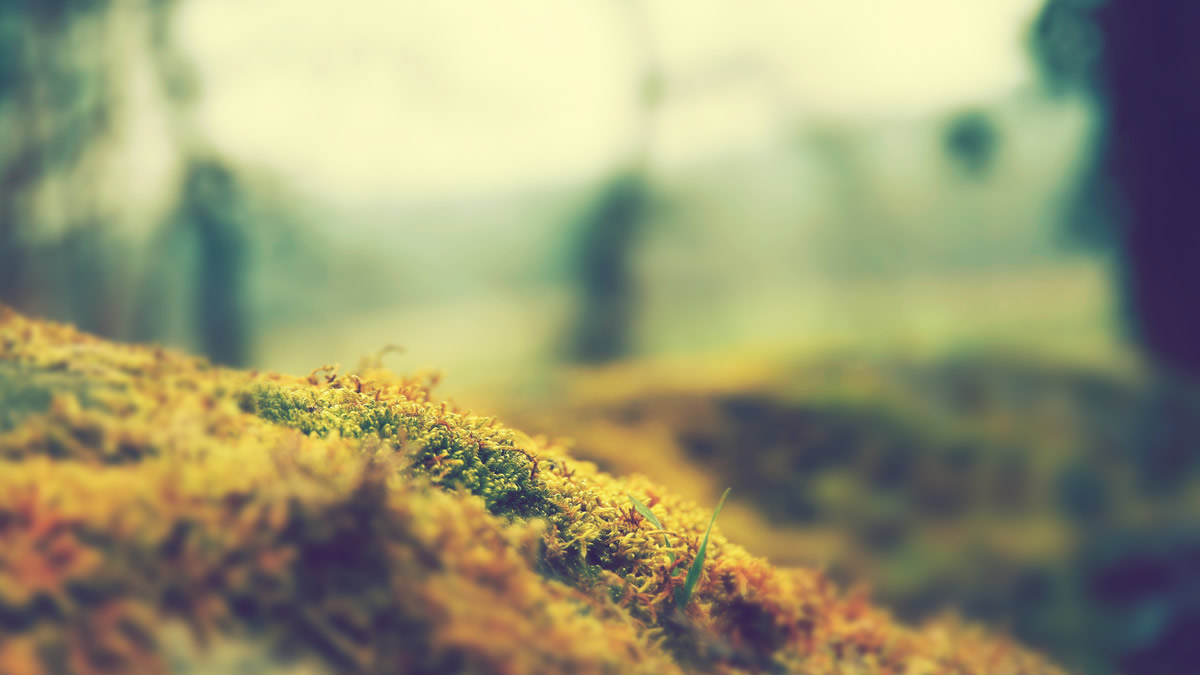
\includegraphics[width=\paperwidth,height=\paperheight]{img/blurry3.jpg}}
\begin{frame}
\begin{center}

\textbf{ATTACKS?}
\end{center}
\end{frame}

%
\fontsize{14pt}{15.2}\selectfont
\usebackgroundtemplate{}
\begin{frame}

On the implementation or on the mathematics.\\\vspace{1cm}
\pause
 \textbf{Model}:

\begin{itemize}
	\item{Recover the plaintext $m^e = c \pmod{N}$}
	\item{Recover the private key $d$}
\end{itemize}
\vspace{1cm}
\pause
\textbf{Relaxed model}:
\pause
\begin{itemize}
	\item{We know a part of the message}
	\item{We know an approximation of one of the prime}
	\item{The private exponent is too small}
\end{itemize}
\end{frame}

% LATTICE
\fontsize{90pt}{15.2}\selectfont
\usebackgroundtemplate{
\includegraphics[width=\paperwidth,height=\paperheight]{img/blurry4.jpg}}
\begin{frame}
\begin{center}

\textbf{LATTICE?}
\end{center}
\end{frame}

% VECTOR SPACE
\fontsize{16pt}{15.2}\selectfont
\usebackgroundtemplate{}
\begin{frame}

A bit like a \textbf{vector space}.\vspace{1cm}

\begin{tikzpicture}[scale=.45]
\draw [lightgray] [<->] (0,5) -- (10,5);
\draw [lightgray] [<->] (5,10) -- (5,0);
\draw [thick,purple] [->] (5,5) -- (6, 8);
\draw [thick,purple] [->] (5,5) -- (6, 6);
\pause
\draw [thick,black] [->] (11,5) -- (12,5);

\draw [lightgray] [<->] (13,5) -- (23,5);
\draw [lightgray] [<->] (18,10) -- (18,0);
%\path [fill=purple] (18,5) to (20.5,10) to (23,10) to (18,5);
\path [fill=purple] (15.5,0) to (20.5,10) to (23,10) to (13,0);
\end{tikzpicture}\\
\end{frame}

\begin{frame}

\begin{figure}[!h]
\centering
\begin{tikzpicture}[scale=.5]
\draw [lightgray] [<->] (0,5) -- (10,5);
\draw [lightgray] [<->] (5,10) -- (5,0);

\draw [fill,purple] (9,1) circle [radius=0.1];

\draw [fill,purple] (7,1) circle [radius=0.1];
\draw [fill,purple] (8,2) circle [radius=0.1];
\draw [fill,purple] (9,3) circle [radius=0.1];

\draw [fill,purple] (5,1) circle [radius=0.1];
\draw [fill,purple] (6,2) circle [radius=0.1];
\draw [fill,purple] (7,3) circle [radius=0.1];
\draw [fill,purple] (8,4) circle [radius=0.1];
\draw [fill,purple] (9,5) circle [radius=0.1];

\draw [fill,purple] (3,1) circle [radius=0.1];
\draw [fill,purple] (4,2) circle [radius=0.1];
\draw [fill,purple] (5,3) circle [radius=0.1];
\draw [fill,purple] (6,4) circle [radius=0.1];
\draw [fill,purple] (7,5) circle [radius=0.1];
\draw [fill,purple] (8,6) circle [radius=0.1];
\draw [fill,purple] (9,7) circle [radius=0.1];

\draw [fill,purple] (1,1) circle [radius=0.1];
\draw [fill,purple] (2,2) circle [radius=0.1];
\draw [fill,purple] (3,3) circle [radius=0.1];
\draw [fill,purple] (4,4) circle [radius=0.1];
\draw [fill,purple] (5,5) circle [radius=0.1];
\draw [fill,purple] (6,6) circle [radius=0.1];
\draw [fill,purple] (7,7) circle [radius=0.1];
\draw [fill,purple] (8,8) circle [radius=0.1];
\draw [fill,purple] (9,9) circle [radius=0.1];

\draw [fill,purple] (1,3) circle [radius=0.1];
\draw [fill,purple] (2,4) circle [radius=0.1];
\draw [fill,purple] (3,5) circle [radius=0.1];
\draw [fill,purple] (4,6) circle [radius=0.1];
\draw [fill,purple] (5,7) circle [radius=0.1];
\draw [fill,purple] (6,8) circle [radius=0.1];
\draw [fill,purple] (7,9) circle [radius=0.1];

\draw [fill,purple] (1,5) circle [radius=0.1];
\draw [fill,purple] (2,6) circle [radius=0.1];
\draw [fill,purple] (3,7) circle [radius=0.1];
\draw [fill,purple] (4,8) circle [radius=0.1];
\draw [fill,purple] (5,9) circle [radius=0.1];

\draw [fill,purple] (1,7) circle [radius=0.1];
\draw [fill,purple] (2,8) circle [radius=0.1];
\draw [fill,purple] (3,9) circle [radius=0.1];

\draw [fill,purple] (1,9) circle [radius=0.1];
\end{tikzpicture}
\end{figure}
\end{frame}

\begin{frame}
\textbf{LLL}, a lattice basis reduction algorithm
\vspace{1cm}

\begin{tikzpicture}[scale=.45]
\node [above] at (5,10) {\textbf{random basis}};
\draw [lightgray] [<->] (0,5) -- (10,5);
\draw [lightgray] [<->] (5,10) -- (5,0);

\draw [fill,purple,opacity=.4] (9,1) circle [radius=0.1];

\draw [fill,purple,opacity=.4] (7,1) circle [radius=0.1];
\draw [fill,purple,opacity=.4] (8,2) circle [radius=0.1];
\draw [fill,purple,opacity=.4] (9,3) circle [radius=0.1];

\draw [fill,purple,opacity=.4] (5,1) circle [radius=0.1];
\draw [fill,purple,opacity=.4] (6,2) circle [radius=0.1];
\draw [fill,purple,opacity=.4] (7,3) circle [radius=0.1];
\draw [fill,purple,opacity=.4] (8,4) circle [radius=0.1];
\draw [fill,purple,opacity=.4] (9,5) circle [radius=0.1];

\draw [fill,purple,opacity=.4] (3,1) circle [radius=0.1];
\draw [fill,purple,opacity=.4] (4,2) circle [radius=0.1];
\draw [fill,purple,opacity=.4] (5,3) circle [radius=0.1];
\draw [fill,purple,opacity=.4] (6,4) circle [radius=0.1];
\draw [fill,purple,opacity=.4] (7,5) circle [radius=0.1];
\draw [fill,purple,opacity=.4] (8,6) circle [radius=0.1];
\draw [fill,purple,opacity=.4] (9,7) circle [radius=0.1];

\draw [fill,purple,opacity=.4] (1,1) circle [radius=0.1];
\draw [fill,purple,opacity=.4] (2,2) circle [radius=0.1];
\draw [fill,purple,opacity=.4] (3,3) circle [radius=0.1];
\draw [fill,purple,opacity=.4] (4,4) circle [radius=0.1];
\draw [fill,purple,opacity=.4] (5,5) circle [radius=0.1];
\draw [fill,purple,opacity=.4] (6,6) circle [radius=0.1];
\draw [fill,purple,opacity=.4] (7,7) circle [radius=0.1];
\draw [fill,purple,opacity=.4] (8,8) circle [radius=0.1];
\draw [fill,purple,opacity=.4] (9,9) circle [radius=0.1];

\draw [fill,purple,opacity=.4] (1,3) circle [radius=0.1];
\draw [fill,purple,opacity=.4] (2,4) circle [radius=0.1];
\draw [fill,purple,opacity=.4] (3,5) circle [radius=0.1];
\draw [fill,purple,opacity=.4] (4,6) circle [radius=0.1];
\draw [fill,purple,opacity=.4] (5,7) circle [radius=0.1];
\draw [fill,purple,opacity=.4] (6,8) circle [radius=0.1];
\draw [fill,purple,opacity=.4] (7,9) circle [radius=0.1];

\draw [fill,purple,opacity=.4] (1,5) circle [radius=0.1];
\draw [fill,purple,opacity=.4] (2,6) circle [radius=0.1];
\draw [fill,purple,opacity=.4] (3,7) circle [radius=0.1];
\draw [fill,purple,opacity=.4] (4,8) circle [radius=0.1];
\draw [fill,purple,opacity=.4] (5,9) circle [radius=0.1];

\draw [fill,purple,opacity=.4] (1,7) circle [radius=0.1];
\draw [fill,purple,opacity=.4] (2,8) circle [radius=0.1];
\draw [fill,purple,opacity=.4] (3,9) circle [radius=0.1];

\draw [fill,purple,opacity=.4] (1,9) circle [radius=0.1];
\draw [thick,purple] [->] (5,5) -- (7, 9);
\draw [thick,purple] [->] (5,5) -- (6, 8);
\pause
%
\node [above] at (18,10) {\textbf{reduced basis}};
\draw [thick,black] [->] (11,5) -- (12,5);
\node [above] at (11.5,5) {$_{LLL}$};
%

\draw [lightgray] [<->] (13,5) -- (23,5);
\draw [lightgray] [<->] (18,10) -- (18,0);

\draw [fill,purple,opacity=.4] (22,1) circle [radius=0.1];

\draw [fill,purple,opacity=.4] (20,1) circle [radius=0.1];
\draw [fill,purple,opacity=.4] (21,2) circle [radius=0.1];
\draw [fill,purple,opacity=.4] (22,3) circle [radius=0.1];

\draw [fill,purple,opacity=.4] (18,1) circle [radius=0.1];
\draw [fill,purple,opacity=.4] (19,2) circle [radius=0.1];
\draw [fill,purple,opacity=.4] (20,3) circle [radius=0.1];
\draw [fill,purple,opacity=.4] (21,4) circle [radius=0.1];
\draw [fill,purple,opacity=.4] (22,5) circle [radius=0.1];

\draw [fill,purple,opacity=.4] (16,1) circle [radius=0.1];
\draw [fill,purple,opacity=.4] (17,2) circle [radius=0.1];
\draw [fill,purple,opacity=.4] (18,3) circle [radius=0.1];
\draw [fill,purple,opacity=.4] (19,4) circle [radius=0.1];
\draw [fill,purple,opacity=.4] (20,5) circle [radius=0.1];
\draw [fill,purple,opacity=.4] (21,6) circle [radius=0.1];
\draw [fill,purple,opacity=.4] (22,7) circle [radius=0.1];

\draw [fill,purple,opacity=.4] (14,1) circle [radius=0.1];
\draw [fill,purple,opacity=.4] (15,2) circle [radius=0.1];
\draw [fill,purple,opacity=.4] (16,3) circle [radius=0.1];
\draw [fill,purple,opacity=.4] (17,4) circle [radius=0.1];
\draw [fill,purple,opacity=.4] (18,5) circle [radius=0.1];
\draw [fill,purple,opacity=.4] (19,6) circle [radius=0.1];
\draw [fill,purple,opacity=.4] (20,7) circle [radius=0.1];
\draw [fill,purple,opacity=.4] (21,8) circle [radius=0.1];
\draw [fill,purple,opacity=.4] (22,9) circle [radius=0.1];

\draw [fill,purple,opacity=.4] (14,3) circle [radius=0.1];
\draw [fill,purple,opacity=.4] (15,4) circle [radius=0.1];
\draw [fill,purple,opacity=.4] (16,5) circle [radius=0.1];
\draw [fill,purple,opacity=.4] (17,6) circle [radius=0.1];
\draw [fill,purple,opacity=.4] (18,7) circle [radius=0.1];
\draw [fill,purple,opacity=.4] (19,8) circle [radius=0.1];
\draw [fill,purple,opacity=.4] (20,9) circle [radius=0.1];

\draw [fill,purple,opacity=.4] (14,5) circle [radius=0.1];
\draw [fill,purple,opacity=.4] (15,6) circle [radius=0.1];
\draw [fill,purple,opacity=.4] (16,7) circle [radius=0.1];
\draw [fill,purple,opacity=.4] (17,8) circle [radius=0.1];
\draw [fill,purple,opacity=.4] (18,9) circle [radius=0.1];

\draw [fill,purple,opacity=.4] (14,7) circle [radius=0.1];
\draw [fill,purple,opacity=.4] (15,8) circle [radius=0.1];
\draw [fill,purple,opacity=.4] (16,9) circle [radius=0.1];

\draw [fill,purple,opacity=.4] (14,9) circle [radius=0.1];

% vectors

\draw [thick,purple] [->] (18,5) -- (19, 4);
\draw [thick,purple] [->] (18,5) -- (19, 6);
\end{tikzpicture}\\

\end{frame}

% basis
\begin{frame}

\begin{center}
\begin{tikzpicture}
\node at (0,0) {$B = \begin{pmatrix}
\vec{b_1}\\
\vdots\\
\vec{b_n}
\end{pmatrix}$};

\draw [->] (1.5,0) -- (3,0) node [above] {\textbf{LLL}} -- (4.5,0);

\node at (6,0) {$B' = \begin{pmatrix}
\vec{b_1'}\\
\vdots\\
\vec{b_n'}
\end{pmatrix}$};

\end{tikzpicture}
\end{center}

 \pause

\[ \|b_1'\| \leq \|b_2'\| \leq \hdots \leq \|b_i'\| \leq 2^{\frac{n(n-1)}{4(n+1-i)}} \cdot det(L)^{\frac{1}{n+1-i}} \]
\end{frame}

% COPPERSMITH
\fontsize{35pt}{15.2}\selectfont
\usebackgroundtemplate{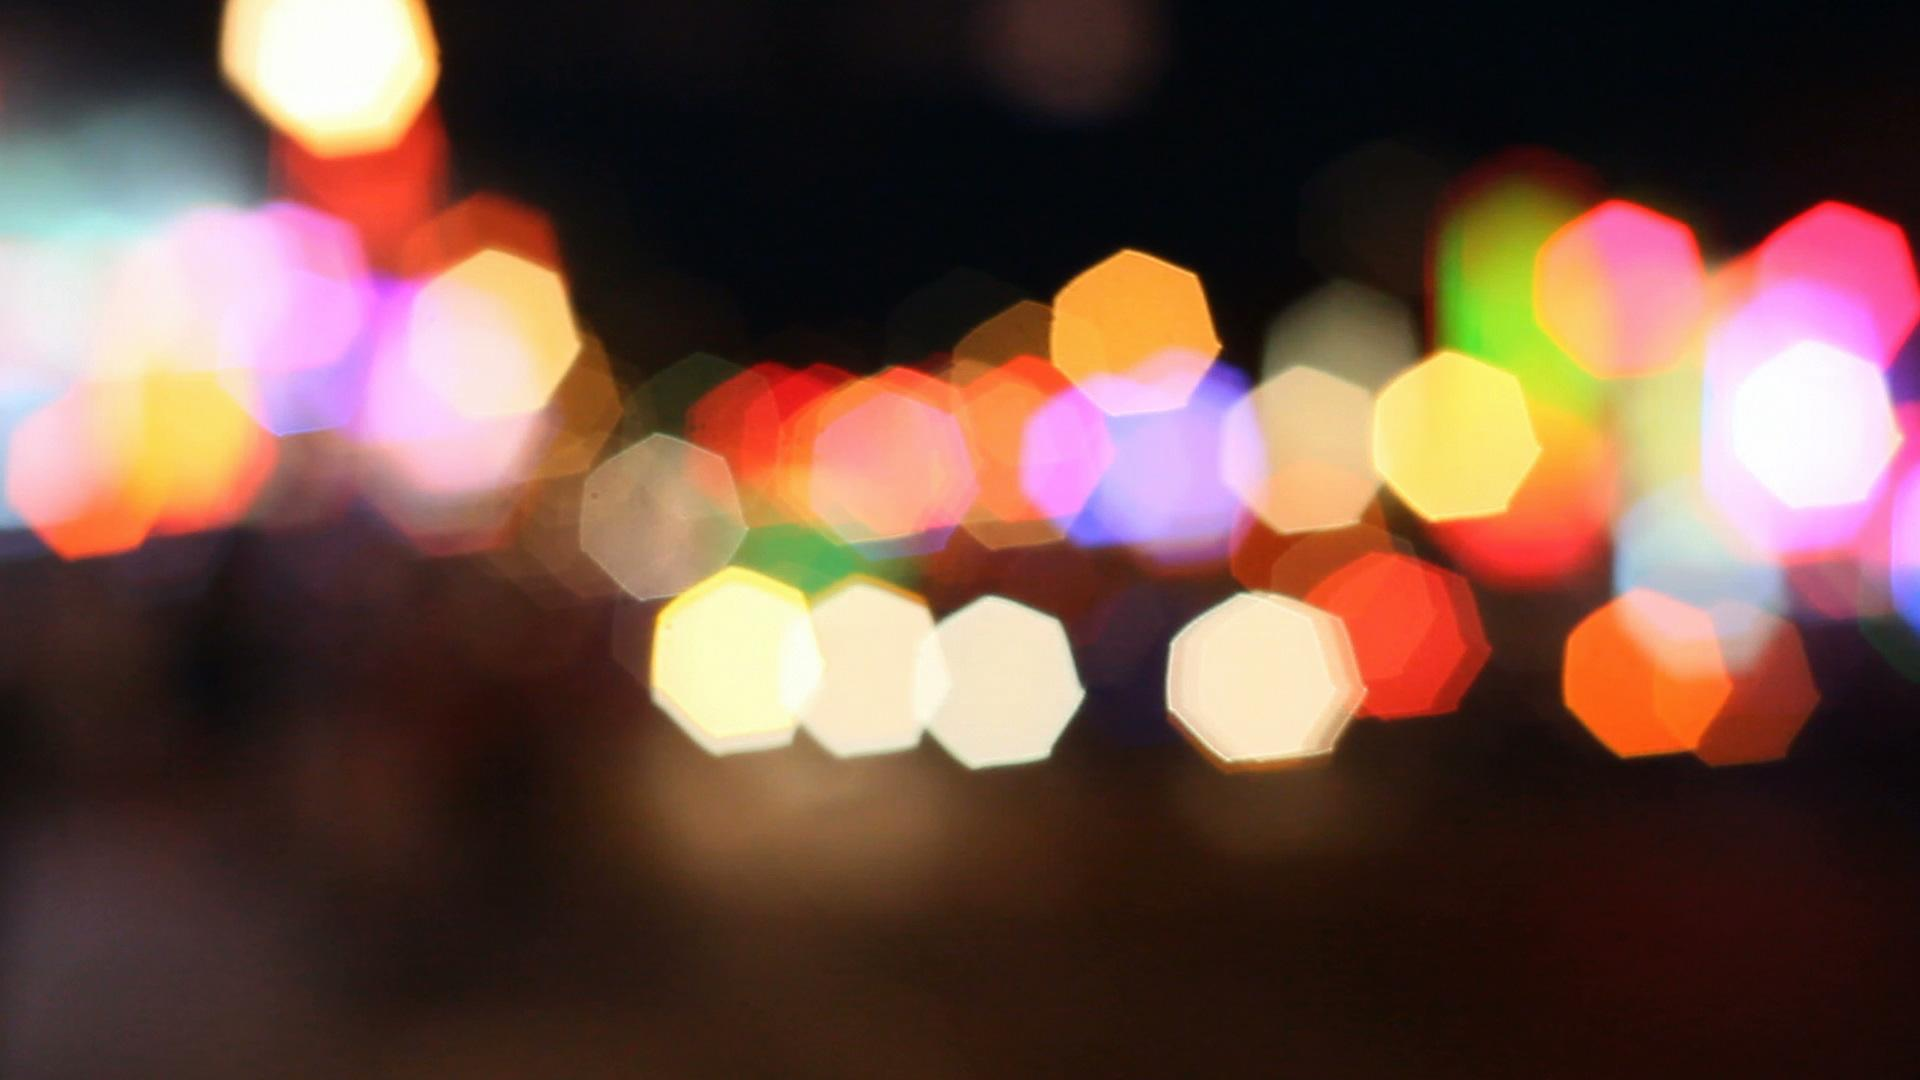
\includegraphics[width=\paperwidth,height=\paperheight]{img/blurry5.jpg}}
\begin{frame}
\begin{center}

\textbf{COPPERSMITH?}
\end{center}
\end{frame}

% STEREOTYPED ATTACK
\fontsize{16pt}{15.2}\selectfont
\usebackgroundtemplate{}
\begin{frame}
\[c = m^e \pmod{N} \]
\pause
\[m = m_0 + x_0\]\\ \vspace{.5cm}
\pause
``le mot de pass du jour est : cupcake''\\
\pause
\[c = (m_0 + x)^e \pmod{N} \]\\
\pause
\[ f(x) = c - (m_0 + x)^e \pmod{N} \]
\end{frame}

% f modulo N -> g over Z
\begin{frame}
\begin{tikzpicture}
\node (A) at (0,2) {$f(x) = 0 \pmod{N}$ with $|x| < X$};
\node (B) at (0,0) {$g(x) = 0$ over $\mathbb{Z}$};
\draw [->,purple] (A) -- (B);
\end{tikzpicture}
\end{frame}

% HOWGRAVE-GRAHAM
\fontsize{14pt}{15.2}\selectfont
\begin{frame}
\textbf{Howgrave-Graham}: \\
Let $g(x)$ be an univariate polynomial with $n$ monomials. Further, let $m$ be a positive integer. Suppose that\pause 
\setcounter{equation}{0}
\begin{align}
&g(x_0) = 0 \pmod{N} \hspace{2mm} \text{ where } \hspace{2mm} |x_0| \leq X
\end{align}

\end{frame}


\begin{frame}
\textbf{Howgrave-Graham}: \\
Let $g(x)$ be an univariate polynomial with $n$ monomials. Further, let $m$ be a positive integer. Suppose that
\setcounter{equation}{0}
\begin{align}
&g(x_0) = 0 \pmod{N} \hspace{2mm} \text{ where } \hspace{2mm} |x_0| \leq X\\
&\|g(xX)\| < \frac{_{N}}{^{\sqrt{n}}}
\end{align}
\pause
Then $g(x_0)=0$ holds over the integers.
\end{frame}


\begin{frame}
\textbf{Howgrave-Graham}: \\
Let $g(x)$ be an univariate polynomial with $n$ monomials. Further, let $m$ be a positive integer. Suppose that
\setcounter{equation}{0}
\begin{align}
&g(x_0) = 0 \pmod{N^m} \hspace{2mm} \text{ where } \hspace{2mm} |x_0| \leq X\\
&\|g(xX)\| < \frac{_{N^m}}{^{\sqrt{n}}}
\end{align}

Then $g(x_0)=0$ holds over the integers.
\end{frame}

% 2nd Diagram using HG
\fontsize{16pt}{15.2}\selectfont
\begin{frame}
\begin{tikzpicture}[scale=1.2]
\node [above] at (2,4) {$f(x_0) = 0 \pmod{N}$ with $|x_0| < X$};
\draw [<-] (0,0) -- (0,4);
\node [below] at (0.6,0) {$g(x_0) = 0$ over $\mathbb{Z}$};
\draw [purple,<-] (0,1) -- (1,1);
\node [right] at (1.2,1.35) {$g(x_0) = 0 \pmod{N^m}$};
\node [right] at (1.2,.65) {$\|g(xX)\| < \frac{N^m}{\sqrt{n}}$};
\draw [purple,<-] (3,2) -- (3,4);
\end{tikzpicture}
\end{frame}

%
\fontsize{14pt}{15.2}\selectfont
\begin{frame}

\textbf{LLL reduction}:
\begin{itemize}
	\item{It only does \textbf{integer linear operations} on the basis vectors}
	\item{The \textbf{shortest vector of the output basis is bound} (as seen in \textbf{Property 1})}\\
\end{itemize}
\end{frame}

% Reminder on LLL property
\begin{frame}
\begin{center}
\begin{tikzpicture}
\node at (0,0) {$B = \begin{pmatrix}
\vec{b_1}\\
\vdots\\
\vec{b_n}
\end{pmatrix}$};

\draw [->] (1.5,0) -- (3,0) node [above] {\textbf{LLL}} -- (4.5,0);

\node at (6,0) {$B' = \begin{pmatrix}
\vec{b_1'}\\
\vdots\\
\vec{b_n'}
\end{pmatrix}$};

\end{tikzpicture}
\end{center}


\[ \|b_1'\| \leq \|b_2'\| \leq \hdots \leq \|b_i'\| \leq 2^{\frac{n(n-1)}{4(n+1-i)}} \cdot det(L)^{\frac{1}{n+1-i}} \]

\pause

\[ \|b_1'\| \leq 2^{\frac{n(n-1)}{4(n)}} \cdot det(L)^{\frac{1}{n}} \]

\end{frame}

% polynomials f_i
\fontsize{16pt}{0}\selectfont
\begin{frame}

\begin{align*}
	g_{i,j}(x) &= x^j \cdot N^i \cdot f^{m-i}(x)\\
	& \text{ for } i = 0,\hdots,m-1,\hspace{2mm} j=0,\hdots,\delta-1\\
	h_i(x) &= x^i \cdot f^m(x)\\
	& \text{ for } i = 0,\hdots,t-1
\end{align*}
\pause

Those polynomials achieve two things:
\begin{itemize}
	\item{they have the \textbf{same root} $x_0$ but modulo $N^m$}
	\pause
	\item{each iteration introduce a new polynomial}\\
\end{itemize}
\end{frame}

% Reminder
\begin{frame}
\begin{tikzpicture}[scale=1.2]
\node [above] at (2,4) {$f(x_0) = 0 \pmod{N}$ with $|x_0| < X$};
\draw [<-] (0,0) -- (0,4);
\node [below] at (0.6,0) {$g(x_0) = 0$ over $\mathbb{Z}$};
\draw [purple,<-] (0,1) -- (1,1);
\node [right] at (1.2,1.35) {$g(x_0) = 0 \pmod{N^m}$};
\node [right] at (1.2,.65) {$\|g(xX)\| < \frac{N^m}{\sqrt{n}}$};
\draw [purple,<-] (3,2) -- (3,4);
\end{tikzpicture}
\end{frame}

% 3rd diagram with LLL
\fontsize{12pt}{0}\selectfont
\begin{frame}
\begin{tikzpicture}
\node (A) at (0,0) {$f(x_0) = 0 \pmod{N}$ with $|x_0| < X$};

\node (B) [below=1cm of A, right] {generate $f_i$ s.t. $f_i(x_0) = 0 \pmod{N^m}$};

\node (C) [below=0.5cm of B] {$B = \begin{pmatrix}
  f_i(xX) \\
  \vdots  \\
  f_n(xX)
 \end{pmatrix}$};

\node (D) [below=0.5cm of C] {$B' = \begin{pmatrix}
  b_1 = g(xX) \\
  b_2\\
  \vdots  \\
  b_n
 \end{pmatrix}$};
 
\node (E) [below=.5cm of D] {$g(x_0) = 0 \pmod{N^m} \text{ and } \|g(xX)\| < \frac{N^m}{\sqrt{n}}$};

\node (F) [left=of E] {$g(x_0) = 0$ over $\mathbb{Z}$};

%
\draw [->] (A) -- (F);
\draw [->] (A) -- (B);
\draw [->] (B) -- (C);
\draw [->] (C) -- (D);
\draw [->] (D) -- (E);
\draw [->] (E) -- (F);

%
\node [above=0.3cm of D,right] {LLL};
\end{tikzpicture}
\end{frame}

% unknown modulus
\begin{frame}

Let $g(x)$ be an univariate polynomial with $n$ monomials. Further, let $m$ be a positive integer. Suppose that
\setcounter{equation}{0}
\begin{align}
&g(x_0) = 0 \pmod{b^m} \hspace{2mm} \text{ where } \hspace{2mm} |x_0| \leq X\\
&\|g(xX)\| < \frac{_{b^m}}{^{\sqrt{n}}}
\end{align}

Then $g(x_0)=0$ holds over the integers.
\end{frame}

% Factoring with high bits known
\begin{frame}


\[ |\tilde{p} - p| < N^{\frac{1}{4}} \]

Now we have an equation with one unknown, modulo another unknown:

\[ \tilde{p} = x_0 \pmod{p} \]
\end{frame}

% bounds, theorem
\begin{frame}
\textbf{Coppersmith Theorem} \\
Let $N$ be an integer of unknown factorization, which has a divisor $b \geq N^{\beta}$, $0 < \beta \leq 1$. Let $f(x)$ be a univariate monic polynomial of degree $\delta$ and let $c \geq 1$.\\
Then we can find in time $\mathcal{O}(c\delta^5log^9(N))$ all solutions $x_0$ of the equation

\[ f(x) = 0 \pmod{b} \hspace{2mm} \text{ with } \hspace{2mm} |x_0| \leq c \cdot N^{\frac{\beta^2}{\delta}} \]
\end{frame}

% BONEH-DURFEE
\fontsize{90pt}{15.2}\selectfont
\usebackgroundtemplate{
\includegraphics[width=\paperwidth,height=\paperheight]{img/blurry6.jpg}}
\begin{frame}
\begin{center}

\textbf{BONEH-DURFEE?}
\end{center}
\end{frame}

% problem
\fontsize{16pt}{15.2}\selectfont
\usebackgroundtemplate{}
%
\end{document}